\section{(Public) Events and (Public Event) Callbacks in Android}
This section presents an introduction to the event-driven and callback mechanism in Android. 
Based on that, we define the public events and public event callbacks. 

%In order to facilitate the understanding of the \atk, 
%this section introduces some relevant background on the event-driven and callback mechanism in Android. 

%\subsection{Events and Callbacks}
In Android, events and callbacks are the ways that an app interacts with the Android system and users. 
In this paper, we define an \textit{event} as a situation that can trigger certain program logic to work. 
For instance, the explicit intent broadcast is an event that can trigger the apps receiving it to execute specific code.
In addition, we define a \textit{public event} as an event that can trigger the 
program logics from \emph{more than one apps} to work. 
Correspondingly, an implicit intent broadcast caters the definition of public event since it can be received by multiple apps. 
%Apparently, the public event is the subset of the event.
Furthermore, we define a \textit{callback} as the code~(e.g., a function and a program branch) that is executed after certain event(s) happen(s), 
and the execution is only related to such event(s). For example, an \texttt{onClick} method would only be executed after user clicks a certain button. 

\subsection{Events and Public Events}

According to the sources that events originated from, the events in Android can be categorized into three groups, 
namely \emph{life-cycle} event, \emph{user-driven} event and \emph{system-driven} event. 
As listed in Table~\ref{tab:events}, each category contains public events that may violate the host apps' control confidentiality. 
In the following, we briefly introduce the events and public events in each category. 

\paragraph{Life-cycle event} An app contains multiple \emph{life-cycle} states, and the state is changed as a user launches, pauses and resumes the app. 
When a new state is entered, the corresponding callbacks will be invoked. 
%Android apps spontaneously arouse corresponding callback functions according to the life-cycle step it resides. We call the event that can trigger life-cycle method to execute as life-cycle event. 
For instance, an Activity executes its \texttt{onCreate} function when it is initially loaded, and executes the \texttt{onPause} callback after it loses the screen focus. 
%Life-cycle callbacks are somehow executed 
%along with user's interactions and impacted by users. 

On surface, due to constraint of sandbox mechanism, the life-cycle phrases (Create,Pause,Destroy, etc.) of an given activity seem to be isolated from components belong to other apps. 
However, the event triggering certain life-cycle callbacks like onCreate and onDestroy enables other app to predict it in an indirect way. For example, the event that an activity is launching leads to the onCreate method in that activity executing. We conclude such life-cycle event that can expose the execution trace of certain app in Table 1.



The trigger-events originated by different sources are equipped with different trigger features. For instance, a \textit{low-battery} event would happen only when the rest quantity of battery becomes as low as a pre-defined level, which is irrelevant to user's interaction. We categorize the events lied in Android that can lead to certain invocation of callback as three groups, namely \textit{life-cycle} event, \textit{user-driven} event, and \textit{system-driven} event.

\textbf{Life-cycle event} Android apps spontaneously arouse corresponding callback function according to the life-cycle step it resides. We call the event that can trigger life-cycle method to execute as life-cycle event. For instance, an Activity executes its \textit{onCreate} function when it is initially loaded, and executes the \textit{onPause} callback after it loses the screen focus. Life-cycle callbacks are somehow executed along with user's interactions and impacted by users. On surface, due to constraint of sandbox mechanism, the life-cycle phrases (Create,Pause,Destroy, etc.) of an given activity seem to be isolated from components belong to other apps. However, the event triggering certain life-cycle callbacks like onCreate and onDestroy enables other app to predict it in an indirect way. For example, the event that an activity is launching leads to the onCreate method in that activity executing. We conclude such life-cycle event that can expose the execution trace of certain app in Table 1.

\textbf{User-driven event} User-driven events interact with corresponding Android API in a direct way. User regularly are guided to perform diverse actions on screen, such as tapping, dropping up and down, click, double-click, etc., to operate a new app. Right after capturing an action from users, Android system would react following the  corresponding callback function that reflects the functionality and logic designed by developer. Generally, the user-driven event trigger the code execution of the one getting screen focus, which is hard capture by other apps. However, there still exists some user-driven events unrelated to the screen(e.g., shake action) acting as public events. 

\textbf{System event} System event normally come from the situation a given system status changes. If not specified, system event could be obtained by any app in theory so long as one is granted proper permissions. Generally, the permission granting could hardly attract user's attention for system event such as battery status is insensitive to user. To the end, system event provides an indirect entry for adversary app getting parts of the running process of other apps that implement system-driven callbacks interfaces. Table1 lists parts of system event instances.

\begin{table*}[t]
\centering
 \caption{\label{tab:events}Parts of events and callbacks in Android}
 \begin{tabularx}{\linewidth}{XXXXX} 
  \toprule
  Categories & Event & Callback & Permission & Public \\
  \midrule
  life-cycle & app starting & onCreate/onStart(launching activity); statical broadcast receiver & N/A & Y\\
             & activity losing focus & onPause & N/A & N\\
             & service starting & onCreate/onBind & N/A & Y\\
             
  user-driven & clicking button & onClick & N/A & N\\
              & shaking & onSensorChanged & N/A & Y\\
              
  system  & Intent.ACTION\_BATTERY\_LOW & onReceive & N/A & Y \\
          & Intent.ACTION\_BOOT\_COMPLETED & onReceive & RECEIVE\_BOOT\_COMPLETED & Y \\
  
  \bottomrule
 \end{tabularx}
\end{table*}

\subsubsection{Callback and Components}
Android platform is a kind of open source operating system established by Linux core. Developers could design and develop their own app product on Android in a flexible way, causing Android freely provides a variety of open source libraries and frameworks for developers. Of which, four types of components plays the key role in Android app's construction, namely \textit{Activity}, \textit{Service}, \textit{Broadcast Receiver} and \textit{Content Provider}. \textit{Activity} is designed as a graphical interface for interacting with users. Nevertheless, \textit{Service} is mainly used for handling complex computing job in background without a graphical user interface. \textit{Broadcast Receiver} provides a global listener that could trigger specific code logic when receive relative message. \textit{Content Provider} providers a universal interface for data storage and management, and for sharing data between different components. As a side-effect of user-driven mechanism, Android provides numerous of callback interfaces to be implemented by generic developers. Most of them rely on certain component, which we give greater details in follows.

\textbf{Callback in Activity} 
Most of callbacks in Activity are invoked by user-driven and life-cycle events, causing activity is mainly used for providing a visible graphic interfaces so as to interact with users. As aforementioned, upon the protection of sandbox, these callback statuses are hardly obtained by other apps only if the event triggered by user is irrelevant to screen focus. For instance, a shake action from users would lead to \textit{sensor} related events, which have no especial association with the screen. Besides, some system-driven callbacks are implemented in activity for catering the requirements of functionalities. 

\textbf{Callback in Service} 
Handling program logic and computing tasks in background, Service has no direct interaction with users, which is typically different from Activity. By this means, callbacks from service only come from life-cycle and system statuses. Yet, user's action without screen focus could be an exception, which we will discuss later.

Service life-cycle consists of five callback functions(onCreate, onStartCommand, onBind, onUnbind and onDestroy) but has a simpler life-cycle procedure compared with Activity. Being the same as Activity, these life-cycle callbacks are isolated from components of other apps so that has little utility value for attacker. 

Regularly, most of \textit{Services} are designed to wait for a typical signal and then invoke corresponding callback functions to push their computing result to an output interface, such as a \textit{dialog} or an \textit{Activity}. In general, the signal could be any type of event, invocation from other component or a program condition. If the trigger event belongs to system events, it can be easily obtained by component from other apps. This makes possible for attackers to perceive the execution process of a target app.

It is also possible to trigger a callback through a user-driven event in service, which is irrelevant to visible screen (e.g., shaking the phone to trigger SensorChanged event). Without specified receiver, this kind of events could be easily obtained by other apps either.   

\textbf{Callback in Broadcast Receiver} 
The \textit{Broadcast} has a wide spectrum of sources, from system or other components and can be delivered across all the installed apps through a common medium \textit{Intent}. Generally, callback functions in Broadcast Receiver only act as a channel that responses the coming Broadcast and then launches corresponding \textit{service} or \textit{activity} to handle it. However, once lacking of strong constraint, Broadcast Receiver could suffer from the threats of repeatedly receiving trash message from an adversary Broadcast sender. Similarly, it is also possible that a typical Broadcast is intercepted by a deliberately designed Receiver. Therefore, developers normally add some protection measures, such as setting the "export" property as false or using self-defined permission, to prevent from such attacks.

\textbf{Callback in Content Provider}
Content Provider acts as a channel for operating database in Android system, so callbacks in Content Provider appear quite trivial. Similar with Service, the Content Provider is designed as background component and its lifecycle callback onCreate() is mainly used to initialize the provider object. However, the provider is initiated when invoked by the operation from ContentResolver related to user-driven and program logic. Therefore, attackers are hard to leverage the process causing the launching time of a certain provider is hard to be captured by other apps. Besides, developers seldom set security related logics within onCreate() and other callbacks of Content Provider. Based on above consideration, we exclude the Content Provider in later PEC discussion.

\section{Exploiting Callbacks}
Android framework provides a variety of callback functions for developers conducting their apps a particular responding after a specific event happens. Yet, abusing these callbacks would incur undesirable consequence as well.
\subsection{Motivating Example}

\begin{figure*}[t]
\centering
\scalebox{1}[0.8]{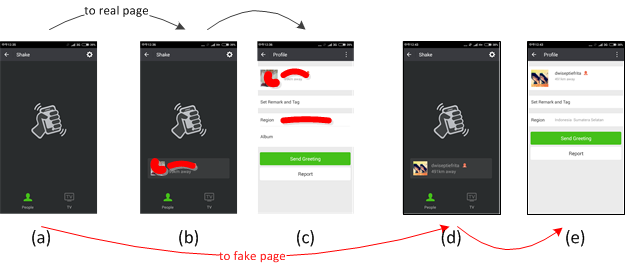
\includegraphics{pic1.png}}
\caption{\label{} Motivating example about the PEC threats. In (a), a user prepare to try the "Shake"; (b) shows a normal case that a real result popped up after shake; (c) presents the further information of such real page after user clicks the result; (d) shows the case that the shake action is perceived by an adversary app, which pop up a fake "result" page after it receives the shake action; (e) presents the further fake information crafted by attacker, which is used to induce user to convince it.}
\end{figure*}

We take the well-known app Wechat as a motivating example. Wechat is known as a popular IM(Instant Messenger) tool for users sharing information and connecting with each other. Of diverse functionalities it provides, "Shake" is rather welcomed, which enables users to randomly obtain an online chatting partner so long as slightly shaking the device several times.

Although harmony in surface, there exists potential crisis in the user shaking action which can be easily perceived by any other app through the {\color{red}SENSOR\_SERVICE}, a system service for managing inner device sensor. That is to say, only with the {\color{red}SystemSensorManager} object instantiation and the arrangement of shaking action size , an adversary app could clearly receive the same action event signal as Wechat. Further more, associating with the running status of Wechat through {\color{red}AMS(Activity Manager Service)}, adversary app could naturally make a judgement about the accurate time when the Wechat responding page would be popped up after user shaking. Although there exists an exception that user could shake the device in other page of "Wechat",the possibility of the exception's emergence is scarcely small in practice because user shakes device in such wide margin normally with intensive intention. {\color{red}Figure 1} shows how the "Shake" event is "stolen" by others. 

It seems that the PEC threats is easily ignored by developers and app markets. We see the callback time leakage severely because it offers a big change for attackers. A wily attacker could devise diverse attacks utilizing the PEC threats. For instants, attackers could deliberately construct a similar result page that links to a malicious third-party chatting tool, or even mimic a fake chatting page to pretend to chat with user for malicious purpose. We presents greater details about the attacks in section **.

\subsection{PEC Model} 

In order to clearly illustrate the callback threats, we view the threats process as a kind of callback state model. Each PEC within a installed app can be described as (S,D,E,C), where "S" denotes current state of app, which can be observed by other apps; "D" denotes the display-sink contained by the callback function; "E" denotes the event that invokes executing of the callback function; "C" denotes the proper control flow conditional values towards the "F".

\paragraph{Component-state}

(s belongs to S)The component-state refers to if the components of an app are running, which provides basic materials to PEC. Similar to the Event, the component-state here also needs to be exposed to other apps.

Before {\color{red}Android 5.0} emerging, the execution state of component like Activity and Service can be easily observed by the {\color{red}getRunningTasks API in ActivityManager object}. A more detailed observation needs to request the "GET\_TASK" permission, which could somehow attract the attention of most of normal users. However, Android starts to constraint the usage of such permission request and the usage of related API from recent {\color{red}Android 5.0+} for the security consideration. The getRunningTasks and even getRunningAppProcess(the API for get all the running process in the device) are now deprecated and only return developer's own application process. {\color{red}A substitute solution is to request new "PACKAGE\_USAGE\_STATS" permission, and to disable warning that permission is system level and will not be granted to third-party apps. Again, this approach needs extra permission request. } A decent solving method to get the foreground running app without any permission request is introduced in  \cite{getforeground} through reading the /proc file where Linux preserves all its process information. For all, obtaining the foreground app is entirely a completable task in common Android system version. 

Another good news is that the usage of  "getRunningServices" are still available in the newest version and need not request any extra permission. Thus, we can judge if a typical service is running through the "getRunningServices" API without any permission request. 

In addition, statically-registered BroadcastReceiver always in the receiving state when the app is running, so its component-state is also easy to ensure. On the other side, the component-state of dynamically-registered BroadcastReceiver follows the running state of its host component, e.g., activity and service, and the method where it is registered.


\paragraph{Display-sink}

(d belongs to D)Display-sink is based on the conception of leakage detection, which refers to a set of label functions that can expose data or information to outside. However, different from traditional conception, Display-sink here specifically refers to state output that could be perceived by users rather than information leakage, including UI page, dialog or notification, etc.

As to the Display-sink, only those output vectors which can be leveraged by attackers are considered. Most of which are related to UI activity, causing the UI is designed as the main channel to interact with users. Some of the UI vectors are mentioned in recent research\cite{bianchi2015app}(e.g., startActivity API, Toast message), yet we also collect some other UI related vectors, e.g., AlertDialog.Builder API, NotificationManager API. Generally, both of Dialog and Notification need response from users(e.g., click) and then engage corresponding reaction functionalities, which offers chance for attackers to interfere the users behaviours, which is insecure.

\textbf{Dialog}
Generally speaking, it goes against Android design and UI guidelines that directly launching a Dialog from Service or BroadcastReceiver. Therefore, if Dialog is roughly created from a Service or BroadcastReceiver, there would pop up an error report causing Dialog is implemented relying on a particular Activity. However, it is pretty work that setting a system alert Dialog with the "SYSTEM\_ALERT\_WINDOW" permission grant. This kind of Dialog has global feature that can be invoked by a Service or a system event rather than an Activity. 

\textbf{Toast}
In common case, the Toast is also constructed based on an existing Activity rather than Service or BroadcastReceiver. The reason of that is one of Toast.makeToast parameters refers to the main UI context the one belongs to. Therefore, directly popping up from Service or BroadcastReceiver would not work causing the UI context is erroneously referred. However, a common-used tool class "Handler" can be used to insert the self-defined thread message into the main thread queue, so that the main thread UI context can be obtained by the Toast. Therefore, Toast can be launched not only in Activity but also in Service and BroadcastReceiver.

\textbf{StartActivity}
The startActivity is known to be invoked by all the three components. However, some Activity is set self-defined permission to improve the security protection. For those low risk "protectionLevel", namely "normal" and "dangerous", we can still apply corresponding self-defined permission to access the target components. Nevertheless, for those high risk level, namely "signature" and "signatureOrSystem", currently there is no any effect way to access the target components by a third party app.

\textbf{Notification}
The Notification can be launched by all the three components as well. Compare to Dialog and Toast, Notification is more likely used in service for notify the task progress or updated information. 



Besides UI sink, some non-UI vectors are also contained, e.g., audio, vibrate related API, sendBroadcast, startService. Similar to UI related vectors, audio and vibrate related API also engage information output although as different information forms("voice and vibration"). The "sendBroadcast" and "startService" is able to lead new callbacks, which threatens the targeted app in a iterative way. Additionally, implicit intent loaded by "sendBroadcast" and "startService" also can be leveraged by attackers.

\paragraph{Event}

(e belongs to E) The event here refers to the public event since non-public one can hardly be exploited by other apps. As mentioned in section **, public events lie in all the three event categories(life-cycle, user-driven and system).

\paragraph{Control Flow}

(C)Control Flow is a collection of conditional values over the path from a typical State to a Display-sink. In theory, as for a callback threat vulnerable app, the "C" needs to guarantee an observable and feasible path that can reach the Display-sink. However, the "C" that strictly conforms above definition rarely emerges in real apps, so that we adopt a more flexible mechanism in practice which will be introduced in next section.  

Attackers need to find a feasible path from the State to the Display-sink within the given operable source code of a target app. For judging the existing of such path, we first collect the condition set of the paths to the Display-sink. Then a signal used to refer to if it is visible for each value, event and function emerging in the condition set is created. To describe more clearly, we denote the following concepts:

1. c: the condition value of each branch.

2. CS: the condition set collected from a program control flow path.

3. cv(a) : the condition value of variable a and a = variable | function | event

4. s(a): the signal value of variable a and a = variable | function | event, whose type is boolean.

s(a) represents if the variable a can be observed by components from other apps. s(a) = true represents yes, s(a) = false represents no.

5. CS = $\cap$ ( cv(a) \& s(a) ) = ($\cap$(c)) \& ( $\cap$ s(a))

Above equation means the value of condition set of a particular path consists of two parts, 1. the value of each variable; 2. the signal value of it. A feasible path needs not only has a solvable condition set, but also observable for each variable. However, practically we normally use the second equation to compute the feasibility of a target path. First, computing out if it is feasible for each branch ; then , considering if it is able to be observed for each variable with the branch condition.

A traditional technique for above computation is symbolic execution. However, it needs unacceptable overhead in practice. {\color {red} To the end, we using an improved SMT approach to solve the constraint conditions.} Normally there should be feasible from source to sink in a target app, otherwise there exists a designation shortage with in the target app. Under this prerequisite, we only need to consider s(a), namely if all the variables are observable. 



%\begin{figure}[t]
%\centering
%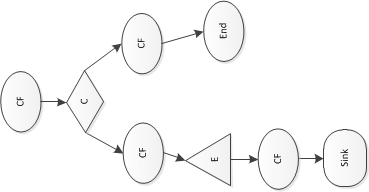
\includegraphics[width = 3.0in]{control-flow.png}
%\caption{\label{}control-flow}
%\end{figure}
%
%\begin{figure}
%\centering
%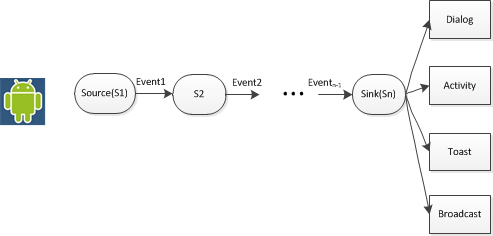
\includegraphics[width = 3.0in]{principle0.png}
%\caption{\label{} principle0}
%\end{figure}
%
%\begin{figure}
%\centering
%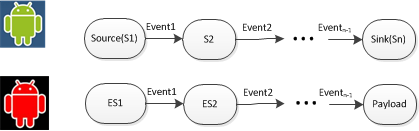
\includegraphics[width = 3.0in]{principle.png}
%\caption{\label{}principle1}
%\end{figure}



\begin{table*}[htbp]
\centering
 \caption{\label{tab:test} Typical vectors of PEC}
 %\begin{tabular}{lcll}
 \begin{tabularx}{\linewidth}{XXXX}

  \toprule
  State & Display-sink & Event & Control Flow \\
  \midrule
 1.Activity running state(Launching page) & 1.startActivity & 1.Broadcast from system: \{Intent.ACTION\_BATTERY\_LOW\} & 1.branch or cycle condition analysis \\
  2. Service running state &2. Toast message & 2.Implicit Intent\& pendingIntent & 2.method invocation analysis\\
     & 3.AlertDialog. Builder & 3.ServiceManager(need not permission grant): { sensorManager, memoryManager }\\
     & 4.sendBroadcast (intent)& 4.ServiceManager(need permission grant): { batteryManager }\\     
     & 5.AudioManager API & \\
     & 6.VibrateManager API & \\
     & 7.NotificationManager API & \\
     
  \bottomrule
 \end{tabularx}
\end{table*}



{\color{red}Table 2} lists the main vulnerability vectors with the callback threats. 
